% =============================================================================
% Template Beamer dos slides da apresentação final do Projeto de Aprendizagem
% de Máquina (pós-graduação), disciplina IN1102. Oferta 2026.2 (release 2026.2.1).
% Repositório-template: projeto-final-IN1102-2026.2.
% Alvo: 20 minutos cronometrados, em dois blocos contíguos de 10 minutos.
% Cerca de 24 frames sugeridos.
% Compilar com: pdflatex slides-tabicl2.tex (duas passadas).
% =============================================================================
\documentclass[aspectratio=169,11pt]{beamer}

% Tema padrão (estável). Caso queira metropolis, descomente:
% \usetheme{metropolis}
\usetheme{Madrid}

\usepackage[utf8]{inputenc}
\usepackage[T1]{fontenc}
\usepackage{lmodern}
\usepackage[brazilian]{babel}
\usepackage{graphicx}
\usepackage{booktabs}
\usepackage{amsmath}
\usepackage{amssymb}
\usepackage{xcolor}
\usepackage{tikz}
\usetikzlibrary{arrows.meta,decorations.pathreplacing,positioning}

\definecolor{cinazul}{RGB}{0, 51, 102}
\definecolor{azulclaro}{RGB}{204, 224, 245}
\definecolor{cinzaescuro}{RGB}{90, 90, 90}
\definecolor{laranja}{RGB}{204, 102, 0}
\definecolor{verdeescuro}{RGB}{0, 102, 51}

% Estilos do diagrama do protocolo (definidos fora dos frames).
\tikzset{
    bloco/.style={minimum height=0.55cm, minimum width=1.5cm, draw=white, line width=0.8pt, inner sep=0pt},
    treino/.style={bloco, fill=azulclaro, text=cinazul},
    teste/.style={bloco, fill=cinzaescuro, text=white},
    etapa/.style={draw=#1, line width=0.8pt, fill=#1!7, rounded corners=2pt, text width=3.4cm, align=center, inner sep=4pt, minimum height=2.4cm, font=\scriptsize},
    seta/.style={-{Stealth[length=2.2mm]}, thick, draw=black!70}
}

\title[Projeto Final de AM (IN1102)]{Projeto Final: Aprendizagem de Máquina (IN1102, pós)}
\subtitle{Modelo tema: \textbf{TabICL v2 (\textit{Tabular In-Context Learning v2})}}
\author[Grupo: \textbf{Douglas, Felipe e Letícia}]{Grupo: \textbf{Douglas Araújo Silva, Felipe Araújo de Lima, Letícia De Albuquerque S.\ Leitão}}
\institute[CIn/UFPE]{Pós-graduação, CIn/UFPE, 2026.2}
\date{Apresentação}

\begin{document}

% Slide 1: capa
% Apresenta: integrante 1
\begin{frame}
    \titlepage
\end{frame}

% Slide 2: agenda
% Apresenta: integrante 1
\begin{frame}{Agenda}
    \textbf{Etapa 1: fundamentação teórica do modelo (10 minutos)}
    \begin{itemize}
        \item Motivação, contexto e intuição
        \item Arquitetura, formulação e forma de aprendizado
        \item Complexidade, hiperparâmetros e posicionamento na literatura
        \item Aplicações e limitações
    \end{itemize}
    \textbf{Etapa 2: estudo experimental (10 minutos)}
    \begin{itemize}
        \item Seleção dos 30 datasets e protocolo de treino, validação e teste
        \item Estudo de overfitting e viés-variância
        \item Resultados no teste e teste de Friedman (Iman-Davenport)
        \item Controle com Holm e Bonferroni-Dunn; Nemenyi e diagrama CD
        \item Padrão vs.\ com busca, regimes, custo e conclusões
    \end{itemize}
\end{frame}

% =====================================================================
% ETAPA 1: 10 minutos
% =====================================================================

% Slide 3: motivação
% Apresenta: integrante 2
\begin{frame}{Etapa 1: motivação e contexto}
    \begin{itemize}
        \item Classificação tabular: \textit{gradient boosting} (XGBoost, LightGBM, CatBoost) ainda é referência pela eficiência e robustez a atributos heterogêneos, escalas irregulares e dados ausentes (Grinsztajn et al., 2022; McElfresh et al., 2023).
        \item Novos paradigmas: modelos de fundação com aprendizado em contexto (\textit{In-Context Learning} --- ICL / PFNs), MLPs modernas (RealMLP, TabM), modelos aditivos (EBM, APLR), métodos de vizinhança (TabR, ModernNCA) e de \textit{kernels} (xRFM).
        \item \textbf{Pergunta:} em quais regimes o modelo \textbf{TabICL v2} é competitivo com LightGBM, XGBoost e CatBoost (\textit{Tuned Defaults} do \texttt{pytabkit})?
    \end{itemize}
    \vspace{0.4em}
    \footnotesize Contexto histórico: das \textit{Prior-Data Fitted Networks} e TabPFN v1/v2 (Hollmann et al., 2023, \textit{Nature} 2025), limitados pelo custo de atenção bidimensional célula a célula $\mathcal{O}(n^2 m + n m^2)$, à decomposição coluna-depois-linha do TabICL v1 (Qu et al., ICML 2025) e ao TabICL v2 (Qu et al., 2026, INRIA Saclay).
\end{frame}

% Slide 4: intuição
% Apresenta: integrante 2
\begin{frame}{Etapa 1: intuição do modelo}
    \begin{columns}[T,onlytextwidth]
        \column{0.55\textwidth}
        \small
        \begin{itemize}
            \setlength{\itemsep}{3pt}
            \item \textbf{Ideia central em uma frase:} transformar o treino rotulado $\mathcal{D}_{\mathrm{tr}}$ em contexto e inferir $P(y_{\mathrm{te}} \mid x_{\mathrm{te}}, \mathcal{D}_{\mathrm{tr}})$ em uma única passagem direta, sem gradientes em \texttt{fit()}.
            \item \textbf{Diferença em relação aos baselines:} GBDTs particionam os eixos iterativamente; o TabICL v2 usa $\approx 33\text{M}$ de pesos congelados e desacopla atenção por coluna e por linha ($\mathrm{TF}_{\mathrm{col}} \to \mathrm{TF}_{\mathrm{row}} \to \mathrm{TF}_{\mathrm{icl}}$), reduzindo o custo de $\mathcal{O}(n^2 m)$ para $\mathcal{O}(n^2 + n m^2)$.
            \item \textbf{Fundamento teórico ou heurístico:} aproximação amortizada da Distribuição Preditiva Posterior (PPD) Bayesiana sob prior de SCMs, Cauchy e kernels de Sobolev.
        \end{itemize}
        \column{0.45\textwidth}
        \centering
        \begin{tikzpicture}[font=\tiny, node distance=0.20cm]
            \node[draw=cinazul, fill=azulclaro!60, rounded corners=2pt, text width=4.3cm, align=center, inner sep=2pt] (in) {\textbf{Entrada tabular concatenada}\\$X = [X_{\mathrm{tr}}; X_{\mathrm{te}}] \in \mathbb{R}^{n \times m},\; y_{\mathrm{tr}}$};
            \node[draw=cinazul, fill=cinazul!8, rounded corners=2pt, text width=4.3cm, align=center, inner sep=2pt, below=of in] (s1) {\textbf{1. $\mathrm{TF}_{\mathrm{col}}$ (Coluna a coluna)}\\Set Transformer ($M=128$)\\$E_{i,j} = x_{i,j} W_{i,j,:} + b_{i,j,:} \in \mathbb{R}^{128}$};
            \node[draw=laranja, fill=laranja!10, rounded corners=2pt, text width=4.3cm, align=center, inner sep=2pt, below=of s1] (s2) {\textbf{2. $\mathrm{TF}_{\mathrm{row}}$ (Interação por linha)}\\RoPE + 4 tokens \texttt{[CLS]}\\Colapsa atributos $\to h_i \in \mathbb{R}^{512}$};
            \node[draw=verdeescuro, fill=verdeescuro!10, rounded corners=2pt, text width=4.3cm, align=center, inner sep=2pt, below=of s2] (s3) {\textbf{3. $\mathrm{TF}_{\mathrm{icl}}$ (Contexto entre linhas)}\\12 camadas + \textbf{QASSMax}\\Inferência em contexto $\to \hat{P}(y_{\mathrm{te}}\mid x_{\mathrm{te}})$};
            \draw[seta] (in) -- (s1);
            \draw[seta] (s1) -- (s2);
            \draw[seta] (s2) -- (s3);
        \end{tikzpicture}
    \end{columns}
\end{frame}

% Slide 5: arquitetura
% Apresenta: integrante 2
\begin{frame}{Etapa 1: arquitetura}
    \centering
    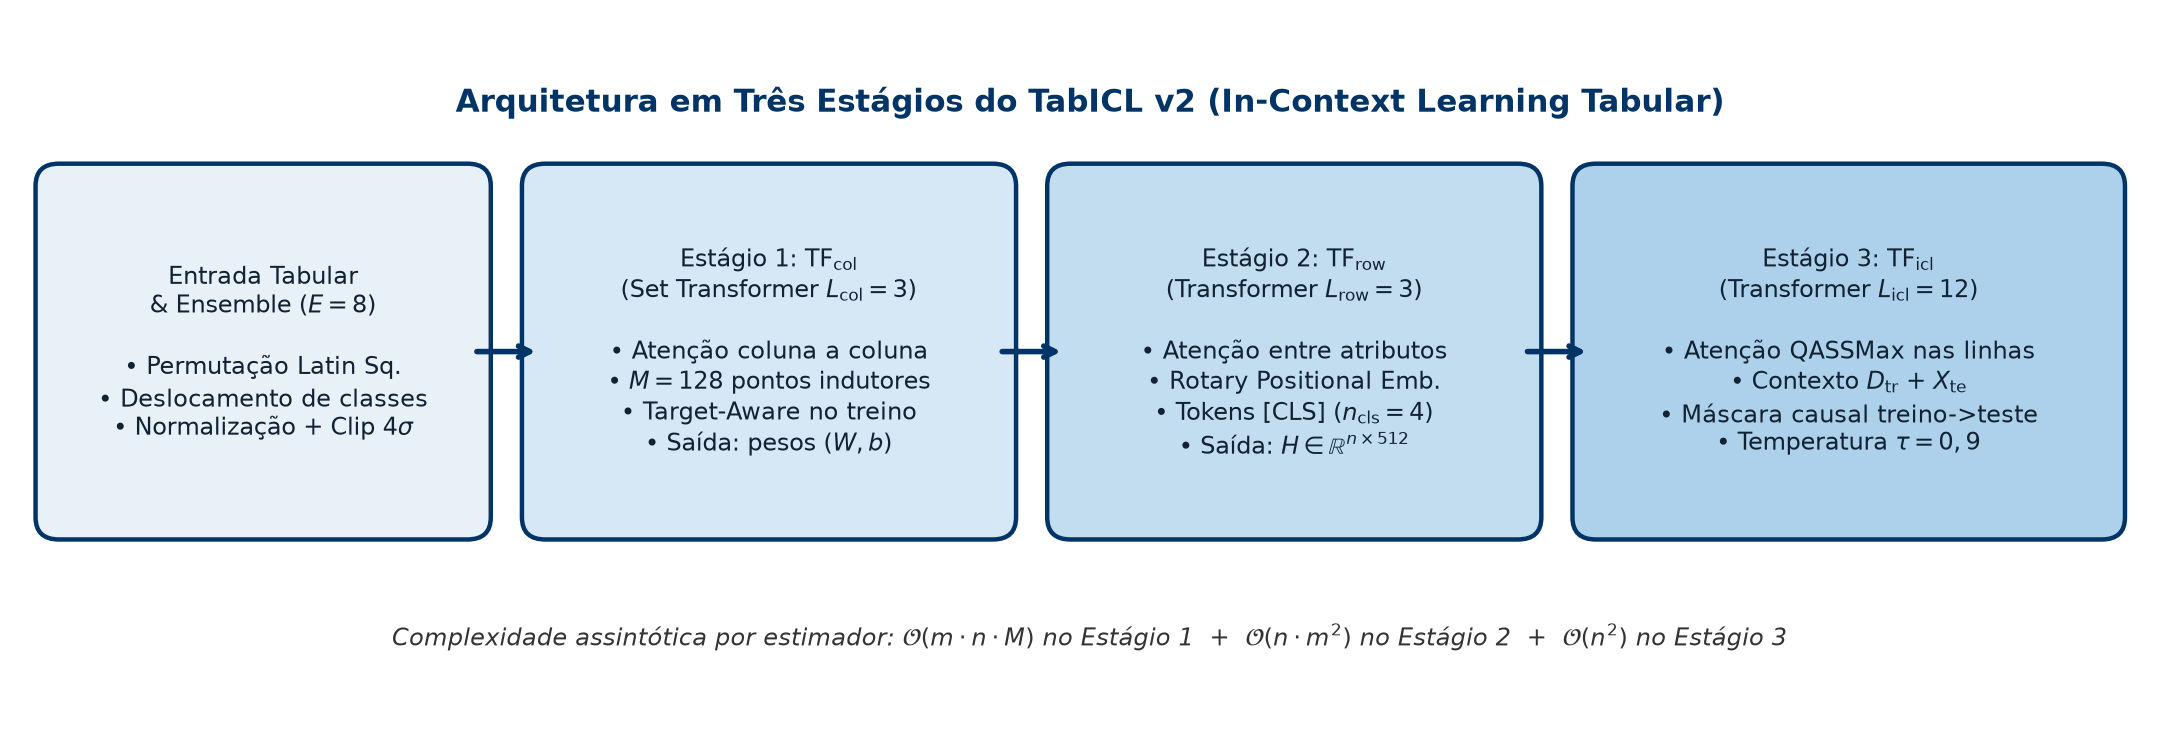
\includegraphics[width=0.90\textwidth]{../figuras/arquitetura_tabicl.png}
    \\[0.3em]
    \scriptsize \textbf{Componentes principais:} \textbf{[Bloco A: $\mathrm{TF}_{\mathrm{col}}$]} $L_{\mathrm{col}}=3$ blocos ISAB ($d_{\mathrm{col}}=128, M=128$, \textit{Repeated Feature Grouping} + \textit{Early Target-Aware Embedding} restrito ao treino) $\to$ transformação afim por célula $E_{i,j} = x_{i,j} W_{i,j,:} + b_{i,j,:}$; \textbf{[Bloco B: $\mathrm{TF}_{\mathrm{row}}$]} $L_{\mathrm{row}}=3$ camadas ($h_{\mathrm{row}}=8$, RoPE) sobre $m+4$ tokens $\to d_{\mathrm{icl}}=512$; \textbf{[Bloco C: $\mathrm{TF}_{\mathrm{icl}}$]} $L_{\mathrm{icl}}=12$ camadas ($h_{\mathrm{icl}}=4$) com escala logarítmica \textbf{QASSMax} $s_{\mathrm{base}}(n_{\mathrm{ctx}}) = 1 + \mathrm{softplus}(\alpha)\log(n_{\mathrm{ctx}})$ e ensemble de $E=8$ visões.
\end{frame}

% Slide 6: formulação e forma de aprendizado
% Apresenta: integrante 3
\begin{frame}{Etapa 1: formulação e forma de aprendizado}
    \small
    \begin{itemize}
        \setlength{\itemsep}{2pt}
        \item \textbf{Função de perda:} no pré-treinamento, minimiza a entropia cruzada esperada sob tarefas sintéticas $D \sim p(\mathcal{T})$: $\mathcal{L}(\theta) = \mathbb{E}_{D}\big[-\sum \log p_\theta(y_{\mathrm{te}} \mid x_{\mathrm{te}}, \mathcal{D}_{\mathrm{tr}})\big]$, aproximando a PPD Bayesiana.
        \item \textbf{Regularização:} prior causal pré-treinado (pesos 100\% congelados na inferência), truncamento simétrico de outliers em $[-\tau_{\mathrm{out}}, +\tau_{\mathrm{out}}]$ e ensemble de $E=8$ visões por quadrados latinos.
        \item \textbf{Como aprende:} pré-treinado offline em $\approx 220\text{M}$ de tabelas sintéticas com otimizador matricial \textbf{Muon} (Newton-Schulz); em dados reais, opera puramente por \textbf{aprendizagem em contexto (ICL)}, com zero gradientes em \texttt{fit()}.
        \item \textbf{Representação dos padrões:} incorporação afim de células no $\mathrm{TF}_{\mathrm{col}}$ ($\mathbb{R}^{128}$), representação condensada por instância no $\mathrm{TF}_{\mathrm{row}}$ ($\mathbb{R}^{512}$) e atenção contextual com QASSMax no $\mathrm{TF}_{\mathrm{icl}}$ (decomposição de base mista se $C > 10$).
        \item \textbf{Categóricos e valores ausentes:} nativo em \texttt{fit()} --- \texttt{OrdinalEncoder} com código ($-1$) para ausentes e categorias não vistas, imputação de ausentes numéricos pela média de $X_{\mathrm{tr}}$ (\texttt{SimpleImputer(strategy="mean")}, sem indicador binário) e normalizações (\texttt{none}, \texttt{power}, \texttt{quantile\_rtdl}).
    \end{itemize}
\end{frame}

% Slide 7: complexidade e memória
% Apresenta: integrante 3
\begin{frame}{Etapa 1: complexidade computacional}
    \footnotesize
    \resizebox{\linewidth}{!}{%
    \begin{tabular}{l c c p{6.0cm}}
        \toprule
        \textbf{Operação} & \textbf{Tempo} & \textbf{Memória} & \textbf{Observação (confronto medido)} \\
        \midrule
        Treino (\texttt{fit}) & $\mathcal{O}(E \cdot n_{\mathrm{tr}} \cdot p)$ & $\mathcal{O}(E \cdot n_{\mathrm{tr}} \cdot p)$ & Apenas visões em CPU; mediana \textbf{1,37 s} (média \textbf{3,86 s}) em \texttt{group\_default} no teste. \\
        \addlinespace[3pt]
        Inferência (\texttt{predict}) & $\mathcal{O}\!\left(E(n p M + n p^2 + n^2)\right)$ & $\mathcal{O}(n p d_{\mathrm{col}} + n p^2 + n^2)$ & Passagem pelos 3 Transformers em GPU; mediana \textbf{3,15 s} (média \textbf{18,38 s}, até $>120\text{ s}$ se $p > 1.600$). \\
        \bottomrule
    \end{tabular}%
    }
    \vspace{0.4em}
    \\
    \footnotesize \textbf{Pico de memória observado:} saturação dos \textbf{15.360 MiB (15 GiB) de VRAM} e RAM paginada (\texttt{exit code 137}) em \texttt{Bioresponse} ($p=1.776$) e \texttt{hiva\_agnostic} ($p=1.617$) na validação, mitigada pelo wrapper \texttt{AdaptiveTabICLClassifier} (\texttt{batch\_size=1} e \texttt{disk\_offload\_dir} quando $p > 500$); alocação de \textbf{$\approx 12,68\text{ GB}$ de VRAM} em \texttt{customer\_satisfaction\_in\_airline} ($n=129.880, n_{\mathrm{te}}=43.293$) no teste; \textbf{hardware:} GPU NVIDIA Tesla T4 (16 GB VRAM, CUDA 12.4) + CPU Intel Xeon.
\end{frame}

% Slide 8: hiperparâmetros
% Apresenta: integrante 3
\begin{frame}{Etapa 1: hiperparâmetros e espaço de busca}
    \scriptsize
    \resizebox{\linewidth}{!}{%
    \begin{tabular}{l p{2.1cm} p{3.6cm} p{5.2cm}}
        \toprule
        \textbf{Hiperparâmetro} & \textbf{Padrão} & \textbf{Faixa de busca (Optuna)} & \textbf{Efeito esperado} \\
        \midrule
        \texttt{norm\_methods} & \texttt{["none","power"]} & 5 combinações categóricas (\texttt{none+power}, \texttt{+robust}, \texttt{+quantile\_rtdl}, \texttt{power}, \texttt{quantile\_rtdl}) & Adapta visões do ensemble a distribuições assimétricas, multimodais ou com caudas pesadas (reduz viés de representação). \\
        \addlinespace[2pt]
        \texttt{outlier\_threshold} & $4{,}0$ & $[2{,}5;\; 6{,}0]$ (contínuo, linear) & Compromisso entre truncar outliers espúrios na atenção ($\tau_{\mathrm{out}}$ baixo) e preservar sinal informativo nas caudas ($\tau_{\mathrm{out}}$ alto). \\
        \addlinespace[2pt]
        \texttt{softmax\_temperature} & $0{,}9$ & $[0{,}5;\; 1{,}5]$ (contínuo, escala log) & Controla a nitidez dos logits antes da agregação; afeta fortemente a entropia cruzada e suaviza probabilidades extremas. \\
        \addlinespace[2pt]
        \texttt{average\_logits} & \texttt{True} & $\{\texttt{True}, \texttt{False}\}$ (categórico) & Combina os $E$ estimadores por produto geométrico normalizado (logits) vs.\ mistura linear de probabilidades. \\
        \addlinespace[2pt]
        \texttt{n\_estimators} & $8$ & Fixo em $8$ na busca (curva: $\{1,2,4,8,16,32\}$) & Reduz monotonicamente a variância de permutação de colunas/classes em proporção linear ao tempo de inferência $\mathcal{O}(E)$. \\
        \bottomrule
    \end{tabular}%
    }
    \\[0.4em]
    \footnotesize \textbf{Fonte das faixas:} artigo original do TabICL v2 (Qu et al., 2026), documentação oficial do \texttt{TabICLClassifier} (\texttt{tabicl 2.2.0}) e literatura de pré-processamento quantílico RTDL (Gorishniy et al., 2021), declaradas em \texttt{docs/declaracoes\_a\_priori.md} sem uso do leaderboard.
\end{frame}

% Slide 9: posicionamento na literatura
% Apresenta: integrante 4
\begin{frame}{Etapa 1: posicionamento na literatura}
    \small
    \begin{itemize}
        \setlength{\itemsep}{2pt}
        \item \textbf{2023:} \textbf{TabPFN v1} (Hollmann et al., ICLR 2023) introduz fundação por ICL em priors de SCMs, restrito a $n \le 1.000, p \le 100$.
        \item \textbf{2024:} \textbf{Tuned Defaults / \texttt{pytabkit}} (Holzmüller et al., NeurIPS 2024) consolida baselines GBDT fortes; \textbf{TabR} (Gorishniy et al., ICLR 2024) integra $k$-NN em redes tabulares treinadas por gradiente.
        \item \textbf{2025:} \textbf{TabPFN v2} (Hollmann et al., \textit{Nature} 2025), benchmark vivo \textbf{TabArena} (Erickson et al., 2025) e \textbf{TabICL v1} (Qu et al., ICML 2025), desacoplando atenção de colunas e linhas.
        \item \textbf{2026:} \textbf{TabICL v2} (Qu et al., fev.\ 2026) lidera TabArena e TALENT superando TabPFN v2/2.5 e GBDTs sem exigir busca de hiperparâmetros.
    \end{itemize}
    \vspace{0.2em}
    \footnotesize \textbf{O modelo TabICL v2 se diferencia por:} (1) complexidade $\mathcal{O}(n^2 + n p^2)$ via colapso por linha e atenção escalável QASSMax; e (2) pré-treinamento aberto (BSD-3-Clause) com otimizador Muon e prior sintético de Cauchy/Sobolev.
\end{frame}

% Slide 10: aplicações e limitações
% Apresenta: integrante 4
\begin{frame}{Etapa 1: aplicações e limitações}
    \small
    \begin{itemize}
        \setlength{\itemsep}{2pt}
        \item \textbf{Aplicações práticas:} classificação tabular de pequeno e médio porte ($n \le 10.000$, $p \le 500$), prototipagem rápida sem HPO (\textit{zero-shot}) e problemas exigindo baixa entropia cruzada (\texttt{group\_default} obteve CE de $0{,}3005$, vencendo em 29/30 bases).
        \item \textbf{Restrições de tamanho ($n$ e $p$ máximos, número de classes):} escala $\mathcal{O}(n p^2)$ exige descarregamento em disco para $p > 500$ (como \texttt{Bioresponse}, $p=1.776$); suporta $C \le 10$ diretamente e $C > 10$ via decomposição hierárquica mista.
        \item \textbf{Suposições sobre os dados (IID, tipos de atributos):} assume instâncias IID no contexto e colunas numéricas ou categóricas/ordinais; não substitui modelos dedicados para texto livre bruto ou séries temporais longas.
        \item \textbf{Requisitos:} requer \textbf{GPU com $\ge 16\text{ GB}$ de VRAM} para inferência rápida ($18{,}38\text{ s}$ médios/fold em GPU vs.\ $0{,}19\text{--}0{,}56\text{ s}$ dos GBDTs em CPU); pesos e código sob licença aberta \textbf{BSD-3-Clause}.
    \end{itemize}
\end{frame}

% =====================================================================
% ETAPA 2: 10 minutos
% =====================================================================

% Slide 11: seleção dos datasets e sistemas
% Apresenta: integrante 5
\begin{frame}{Etapa 2: datasets, sistemas e métricas}
    \small
    \begin{itemize}
        \setlength{\itemsep}{2pt}
        \item \textbf{Datasets:} 30 do TabArena-v0.1 (OpenML 457: 10 pequenos, 10 médios, 10 grandes até $n=129.880$), escolhidos pelo catálogo antes de qualquer resultado (\texttt{check\_selection} ok); \textbf{critério:} equilíbrio entre binários (24) e multiclasse (6), atributos categóricos (15 $<25\%$ e 15 $\ge 25\%$) e dados ausentes (6).
        \item \textbf{Sistemas:} \textbf{TabICL v2 padrão} (\texttt{group\_default}) e \textbf{TabICL v2 com busca} (\texttt{group\_tuned}, controle); \textbf{LightGBM}, \textbf{CatBoost} e \textbf{XGBoost} (\textit{Tuned Defaults} do \texttt{pytabkit}, via \texttt{ImputedClassifier}).
        \item \textbf{Busca:} Optuna (TPE, \texttt{seed=42+fold}) no treino de cada fold externo, 20 tentativas, CV interna de 3 folds, limite de 600 s (tempo efetivo no teste: mediana \textbf{170,67 s}, máx.\ \textbf{717,95 s}), subamostra de até 10.000.
        \item \textbf{Espaço de busca:} 4 hiperparâmetros (\texttt{norm\_methods}, \texttt{outlier\_threshold}, \texttt{softmax\_temperature}, \texttt{average\_logits}) justificados a priori por Qu et al.\ (2026), documentação e Gorishniy et al.\ (2021).
        \item \textbf{Métricas:} \textbf{AUC OvO} (primária), Acurácia (ACC), G-Mean, Entropia Cruzada (CE, secundária) e custo computacional (s).
    \end{itemize}
\end{frame}

% Slide 12: protocolo de treino, validação e teste
% Apresenta: integrante 5
\begin{frame}{Etapa 2: protocolo de treino, validação e teste (CV aninhada)}
    \centering
    \resizebox{\textwidth}{!}{%
    \begin{tikzpicture}[font=\footnotesize]
    \node[anchor=east] at (0.15,0) {Fold externo 0};
    \node[teste]  at (1.05,0) {teste};
    \node[treino] at (2.55,0) {treino};
    \node[treino] at (4.05,0) {treino};
    \node[anchor=east] at (0.15,-0.8) {Fold externo 1};
    \node[treino] at (1.05,-0.8) {treino};
    \node[teste]  at (2.55,-0.8) {teste};
    \node[treino] at (4.05,-0.8) {treino};
    \node[anchor=east] at (0.15,-1.6) {Fold externo 2};
    \node[treino] at (1.05,-1.6) {treino};
    \node[treino] at (2.55,-1.6) {treino};
    \node[teste]  at (4.05,-1.6) {teste};
    \draw[decorate, decoration={brace, amplitude=5pt}, thick] (4.95,0.3) to (4.95,-1.9);
    \node[anchor=west, text width=7.6cm, align=left] at (5.25,-0.8) {%
        \textbf{Treino de cada fold externo:} CV interna de 3 folds com a busca
        e todos os estudos (sensibilidade, específico, curvas, overfitting).\\[2pt]
        \textbf{Teste de cada fold externo:} selado; usado uma única vez.};
    \node[etapa=cinazul] (e1) at (-0.3,-3.75) {%
        \textbf{1. Desenvolvimento}\\[2pt]
        \texttt{run\_validation}, notebooks 02, 03 e 05\\[2pt]
        \texttt{validation.csv} (diagnóstico)};
    \node[etapa=laranja] (e2) at (3.65,-3.75) {%
        \textbf{2. Congelamento}\\[2pt]
        \texttt{freeze} e \texttt{git commit}\\[2pt]
        \texttt{protocolo.lock}: hashes e orçamento};
    \node[etapa=cinzaescuro] (e3) at (7.6,-3.75) {%
        \textbf{3. Avaliação final única}\\[2pt]
        \texttt{final\_test} e \texttt{git commit}\\[2pt]
        \texttt{test.csv}, \texttt{test\_log.csv}; \texttt{check\_protocol}};
    \node[etapa=verdeescuro] (e4) at (11.55,-3.75) {%
        \textbf{4. Análise}\\[2pt]
        média dos 3 testes por dataset\\[2pt]
        Dem\v{s}ar com $N = 30$};
    \draw[seta] (e1) to (e2);
    \draw[seta] (e2) to (e3);
    \draw[seta] (e3) to (e4);
    \end{tikzpicture}}
    \\[0.2em]
    \scriptsize \textbf{Lock:} commit \texttt{9718c9649b} (árvore \texttt{0595782f}, anterior ao 1º commit de resultados \texttt{983c42aa4f}), sha256 \texttt{59901430bd8c...}; \textbf{execuções em \texttt{test\_log.csv}:} 5 (\texttt{1 inicial resume=False + 4 retomadas resume=True} apenas de pendências/OOM, $450/450$ ok); \textbf{\texttt{check\_protocol}:} \textbf{APROVADO}. \textbf{Declarados a priori (\texttt{e2c6968}):} espaço de 4 HPs, bases de estudo (\texttt{363621}, \texttt{363704}, \texttt{363628}) e grades de complexidade.
\end{frame}

% Slide 13: lacuna de generalização
% Apresenta: integrante 5
\begin{frame}{Etapa 2: overfitting, lacuna treino-validação}
    \begin{columns}[T,onlytextwidth]
        \column{0.50\textwidth}
        \scriptsize
        \begin{tabular}{l c c c c}
            \toprule
            \textbf{Sistema} & \textbf{Treino} & \textbf{Val.} & \textbf{Lacuna geral} & \textbf{Peq./Grd.} \\
            \midrule
            TabICL v2 padrão    & $0{,}9505$ & $0{,}8542$ & $0{,}0963 \pm 0{,}0980$ & $0{,}091 / 0{,}082$ \\
            TabICL v2 c/ busca* & $0{,}9511$ & $\mathbf{0{,}8556}$ & $0{,}0955 \pm 0{,}0985$ & $0{,}089 / 0{,}082$ \\
            LightGBM (TD)       & $0{,}9190$ & $0{,}8304$ & $\mathbf{0{,}0886} \pm 0{,}0708$ & $0{,}072 / 0{,}099$ \\
            XGBoost (TD)        & $0{,}9525$ & $0{,}8190$ & $0{,}1335 \pm 0{,}1038$ & $0{,}159 / 0{,}107$ \\
            CatBoost (TD)       & $0{,}9311$ & $0{,}8328$ & $0{,}0983 \pm 0{,}0846$ & $0{,}131 / 0{,}064$ \\
            \bottomrule
        \end{tabular}
        \\[0.3em]
        {\tiny *AUC OvO em 270 partições internas (\texttt{validation\_train.csv} vs.\ \texttt{validation.csv}); em \texttt{group\_tuned}, a validação é otimista (\texttt{optimistic=True}).}
        \column{0.48\textwidth}
        \centering
        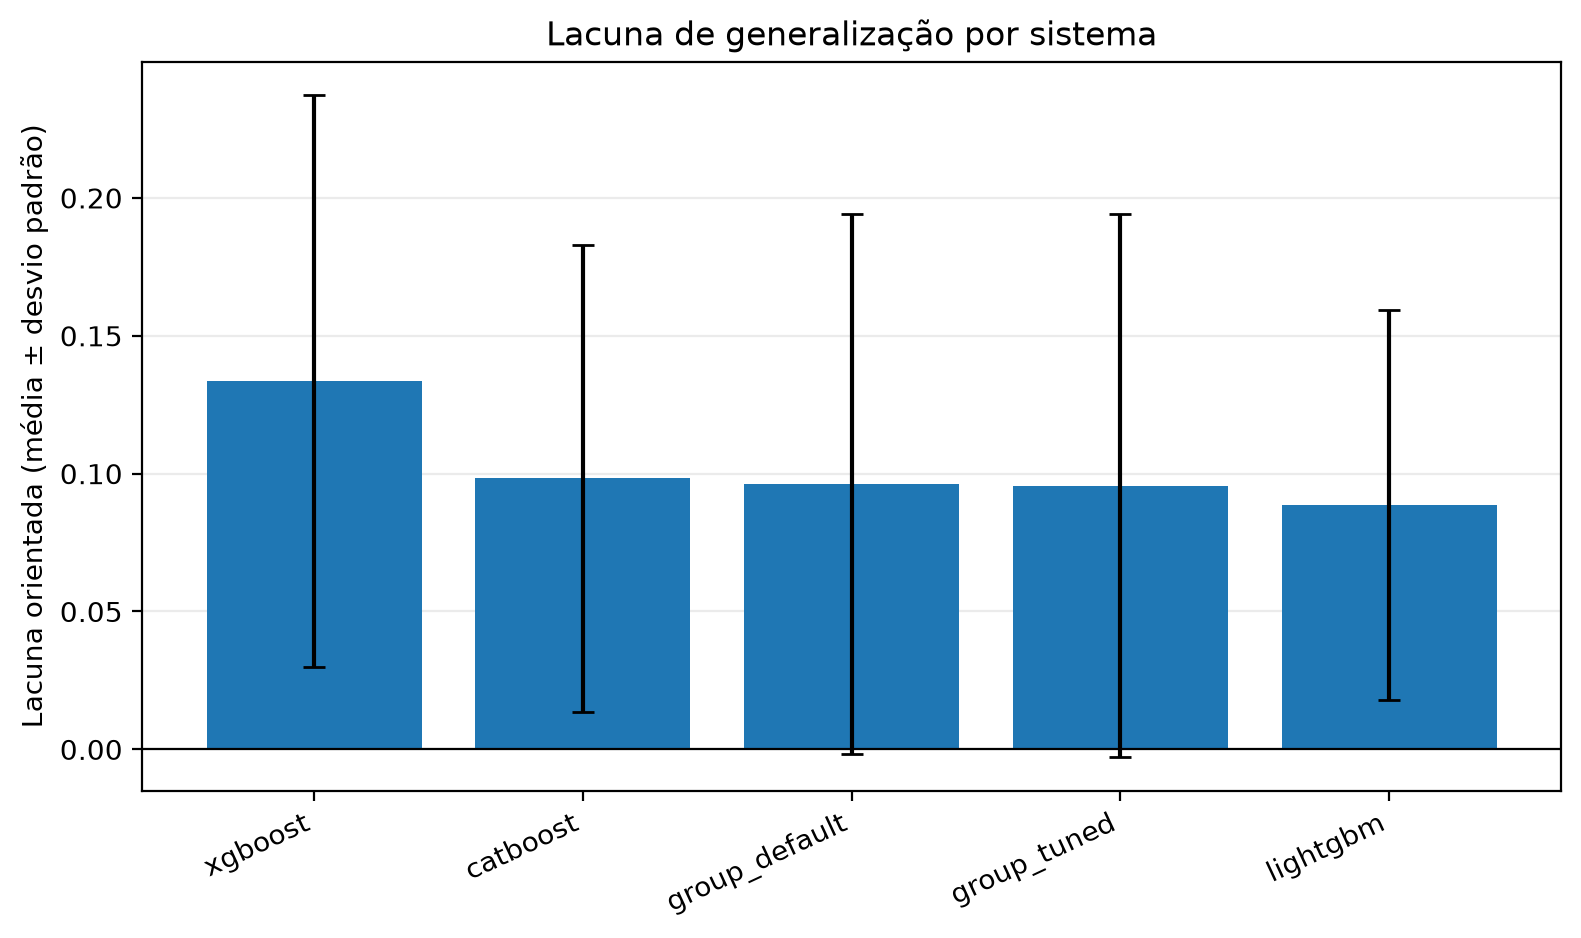
\includegraphics[width=0.95\linewidth]{../../../results/figures/lacuna_auc_ovo.png}
    \end{columns}
    \vspace{0.25em}
    \scriptsize \textbf{Leitura:} maior lacuna ocorre no \textbf{XGBoost ($0{,}1335$)} e \textbf{CatBoost ($0{,}0983$)}, especialmente no regime \textbf{pequeno ($0{,}1585$ e $0{,}1313$)}, onde árvores profundas memorizam ruído amostral ($\text{AUC}_{\mathrm{val}} = 0{,}8056$ no XGBoost pequeno). \textbf{Cautelas:} (1) no TabICL v2, $\text{AUC}_{\mathrm{treino}} \approx 0{,}951$ (medida em subamostra de até 2.000 instâncias) decorre de \textit{in-context lookup} (cada instância consultada já está presente com seu rótulo no contexto do $\mathrm{TF}_{\mathrm{icl}}$), não de ajuste de pesos; e (2) a validação de \texttt{group\_tuned} ($0{,}8556$) tem viés otimista de seleção nos 3 folds internos.
\end{frame}

% Slide 14: curvas de validação e regra de 1 EP
% Apresenta: integrante 5
\begin{frame}{Etapa 2: curvas de validação e regra de 1 erro padrão}
    \begin{columns}[T,onlytextwidth]
        \column{0.49\textwidth}
        \centering
        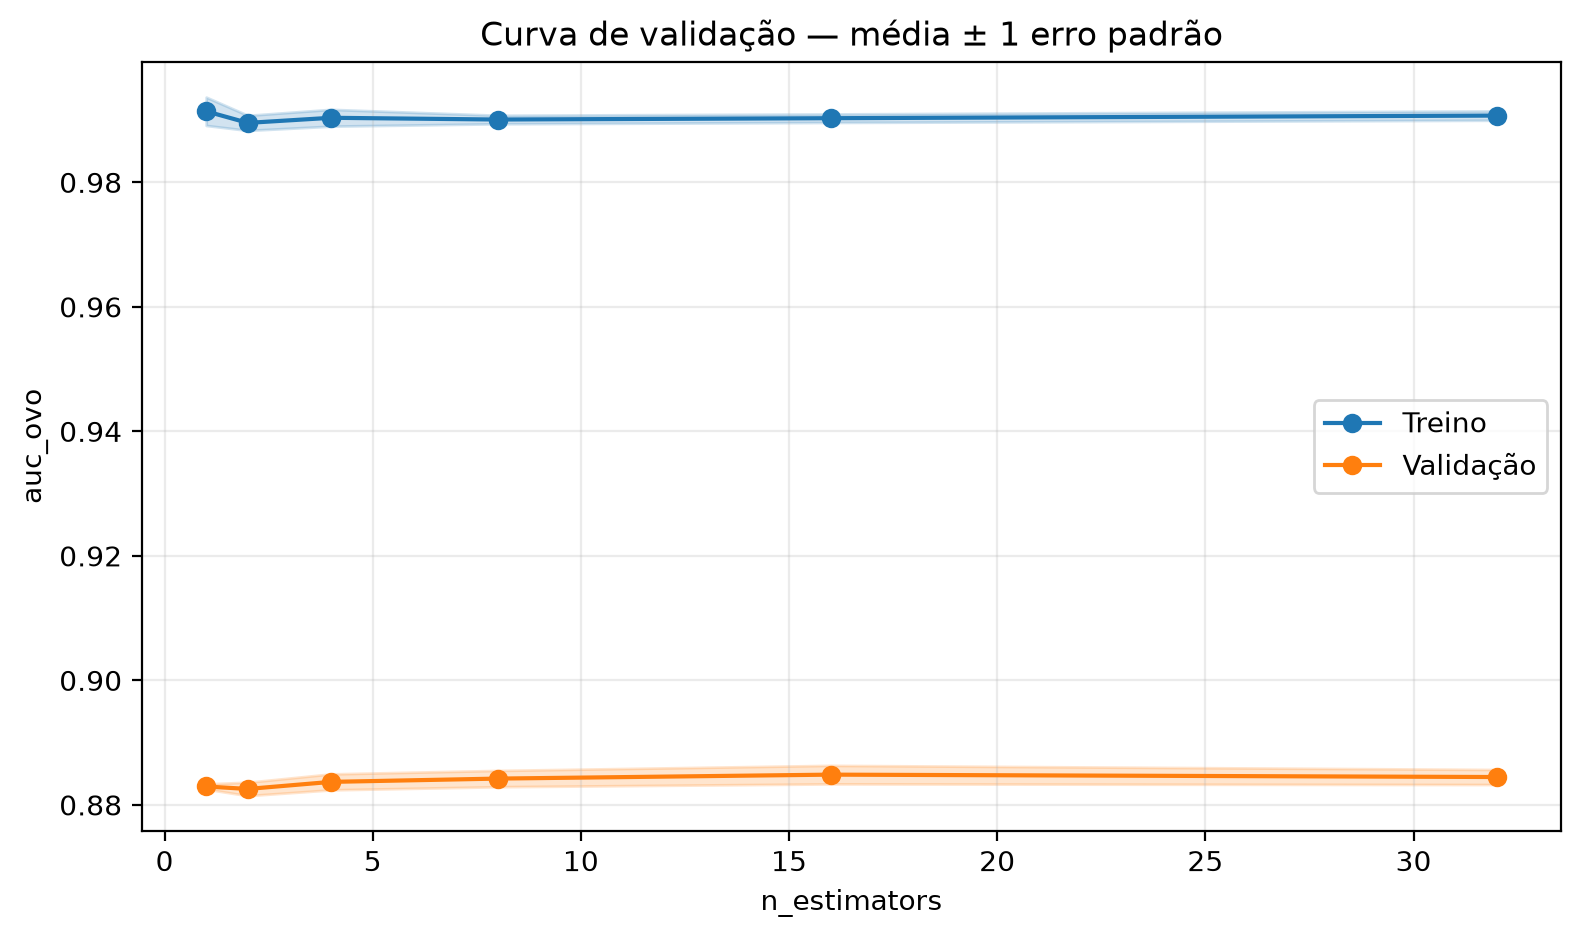
\includegraphics[height=2.45cm]{../../../results/figures/curva_grupo_363704.png}
        \\[-0.2em]
        {\tiny TabICL v2: \texttt{n\_estimators} $\in \{1,2,4,8,16,32\}$ (\texttt{363704}, médio)}
        \column{0.49\textwidth}
        \centering
        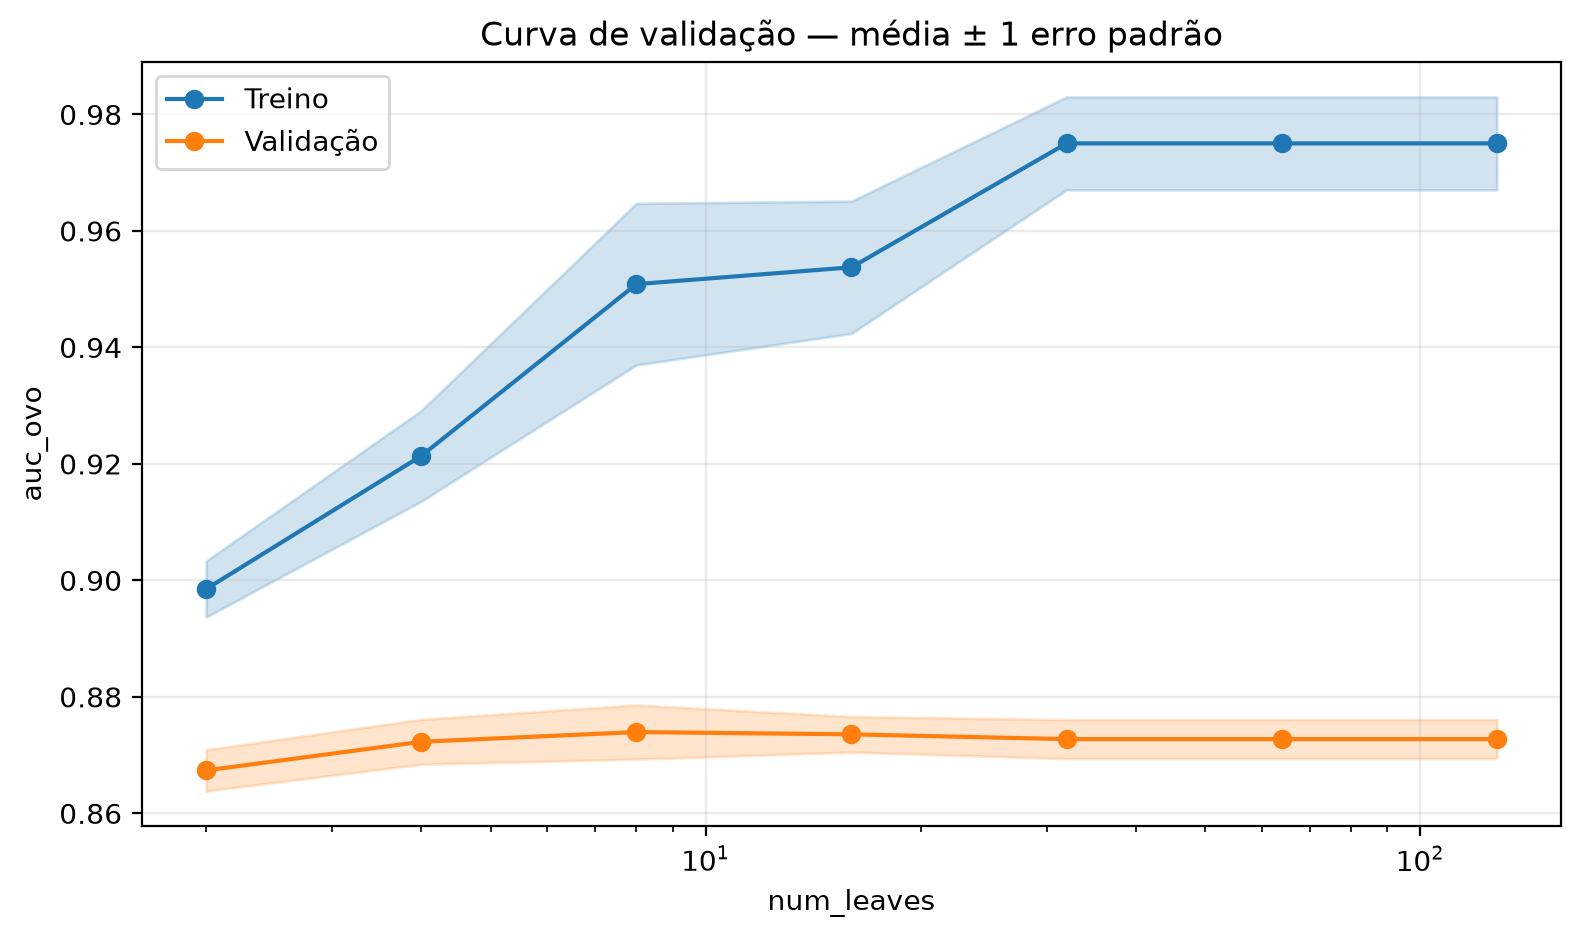
\includegraphics[height=2.45cm]{../../../results/figures/curva_lgbm_363704.png}
        \\[-0.2em]
        {\tiny LightGBM: \texttt{num\_leaves} $\in \{2,4,8,16,32,64,128\}$ (\texttt{363704}, médio)}
    \end{columns}
    \vspace{0.2em}
    \begin{itemize}
        \scriptsize
        \setlength{\itemsep}{1pt}
        \item \textbf{Datasets (declarados a priori, um por regime, CV interna no fold 0):} \texttt{363621} (pequeno, $n=748$), \texttt{363704} (médio, $n=4.424$, 3 classes) e \texttt{363628} (grande, $n=129.880$).
        \item \textbf{Melhor média vs.\ regra de 1 EP (\texttt{SIMPLER\_IS\_LOWER=True}):} TabICL v2 (\texttt{n\_estimators}): melhor média $= \mathbf{16, 16, 32}$ ($0{,}7552 / 0{,}8849 / 0{,}9915$); regra de 1 EP $= \mathbf{1, 4, 1}$ ($0{,}7525 / 0{,}8837 / 0{,}9906$). Fixo a priori em $E=8$ (dentro da banda de 1 EP nos 3 regimes). LightGBM (\texttt{num\_leaves}): melhor média $= \mathbf{4, 8, 16}$; regra de 1 EP $= \mathbf{4, 4, 8}$.
        \item \textbf{Viés e variância:} LightGBM sobreajusta com $\texttt{num\_leaves} > 8$; no TabICL v2, $E=8$ situa-se no platô onde mais estimadores reduzem variância sem inflar viés (treino plano).
        \item \textbf{Erros por classe na validação (\texttt{preds\_val/}):} menor recall na classe minoritária (\texttt{Yes} em \texttt{363621}: $0{,}178$ XGBoost vs.\ $0{,}271$ TabICL; \texttt{Enrolled} em \texttt{363704}: \textbf{$0{,}426$ TabICL} vs.\ $0{,}349$ XGBoost), justificando maior G-Mean do TabICL v2.
    \end{itemize}
\end{frame}

% Slide 15: resultados gerais
% Apresenta: integrante 5
\begin{frame}{Etapa 2: resultados no teste (avaliação final única)}
    \scriptsize
    \centering
    \resizebox{\linewidth}{!}{%
    \begin{tabular}{l c c c c c c}
        \toprule
        \textbf{Sistema} & \textbf{AUC OvO (Teste)} & \textbf{Acurácia} & \textbf{G-Mean} & \textbf{Entropia Cruz.} & \textbf{Posto (AUC)} & \textbf{Tempo Med./Méd. (s)} \\
        \midrule
        \textbf{TabICL v2 padrão}    & $\mathbf{0{,}8607 \pm 0{,}1170}$ & $0{,}8703 \pm 0{,}0878$ & $\mathbf{0{,}6548 \pm 0{,}2915}$ & $\mathbf{0{,}3005 \pm 0{,}1633}$ & N/A ($1{,}20$*) & $\mathbf{4{,}86}$ / $22{,}24$ \\
        \textbf{TabICL v2 c/ busca}  & $0{,}8606 \pm 0{,}1166$ & $\mathbf{0{,}8704 \pm 0{,}0877}$ & $0{,}6541 \pm 0{,}2923$ & $0{,}3150 \pm 0{,}1673$ & $\mathbf{1{,}30}$ & $174{,}72$ / $218{,}78$ \\
        LightGBM (TD)                & $0{,}8407 \pm 0{,}1190$ & $0{,}8570 \pm 0{,}0905$ & $0{,}6187 \pm 0{,}2834$ & $0{,}3447 \pm 0{,}1613$ & $2{,}63$ & $1{,}17$ / $3{,}32$ \\
        CatBoost (TD)                & $0{,}8405 \pm 0{,}1159$ & $0{,}8588 \pm 0{,}0866$ & $0{,}6370 \pm 0{,}2668$ & $0{,}4551 \pm 0{,}2569$ & $2{,}87$ & $4{,}29$ / $4{,}73$ \\
        XGBoost (TD)                 & $0{,}8281 \pm 0{,}1259$ & $0{,}8548 \pm 0{,}0885$ & $0{,}6166 \pm 0{,}2718$ & $0{,}4277 \pm 0{,}2120$ & $3{,}20$ & $1{,}69$ / $2{,}96$ \\
        \bottomrule
    \end{tabular}%
    }
    \\[0.4em]
    \footnotesize \raggedright
    \textbf{Média $\pm$ desvio entre os $N = 30$ datasets completos} (média dos testes dos 3 folds externos por dataset em \texttt{results/test.csv}; *posto de \texttt{group\_default} se comparado aos 3 baselines). \textbf{Incerteza via bootstrap ($B=1.000$):} menor largura mediana de IC 95\% em AUC OvO no TabICL v2 (\textbf{$0{,}0327$} em \texttt{group\_tuned} e \textbf{$0{,}0329$} em \texttt{group\_default} vs.\ $0{,}0388\text{--}0{,}0410$ nos baselines).\\
    \textbf{Validação interna vs.\ teste (AUC OvO):} \texttt{group\_default} subiu de $0{,}8542$ para $0{,}8607$ e \texttt{lightgbm} de $0{,}8304$ para $0{,}8407$ (maior volume de treino externo), mas a vantagem aparente de $+0{,}0014$ de \texttt{group\_tuned} na validação ($0{,}8556$ vs.\ $0{,}8542$, inflada pelo otimismo de seleção) desapareceu no teste selado ($0{,}8606$ vs.\ $0{,}8607$).
\end{frame}

% Slide 16: Friedman com Iman-Davenport
% Apresenta: integrante 5
\begin{frame}{Etapa 2: teste de Friedman com correção de Iman-Davenport}
    \begin{itemize}
        \item \textbf{Configuração experimental:} $k = 4$ sistemas (\texttt{group\_tuned} como controle vs.\ \texttt{lightgbm}, \texttt{catboost}, \texttt{xgboost}), $N = 30$ datasets independentes (média dos 3 folds externos por dataset), nível de significância $\alpha = 0{,}05$.
        \item \textbf{Métrica primária (AUC OvO):} $\chi^2_F = \mathbf{37{,}480}$ ($p = 3{,}642 \times 10^{-8}$, $\text{gl}=3$); estatística corrigida de Iman-Davenport:
        \[
            F_F = \frac{(N - 1)\chi^2_F}{N(k - 1) - \chi^2_F} = \mathbf{20{,}695} \quad \text{com } \mathbf{(3, 87)} \text{ graus de liberdade}; \quad \mathbf{p = 3{,}284 \times 10^{-10}}.
        \]
        \item \textbf{Métrica secundária pré-declarada (Entropia Cruzada):} $\chi^2_F = \mathbf{41{,}640}$ ($p = 4{,}781 \times 10^{-9}$); $F_F = \mathbf{24{,}970}$ com $(3, 87)$ gl; $\mathbf{p = 9{,}532 \times 10^{-12}}$ (postos: \texttt{group\_tuned} $1{,}433$, \texttt{lightgbm} $2{,}133$, \texttt{catboost} $3{,}133$, \texttt{xgboost} $3{,}300$).
        \item \textbf{Decisão (por $F_F$, mais poderosa e menos conservadora que $\chi^2_F$):} \textbf{rejeita-se fortemente a hipótese nula $H_0$} ($p \ll 0{,}05$) em ambas as métricas, habilitando os pós-testes de Holm, Bonferroni-Dunn e Nemenyi.
        \item \textbf{Datasets excluídos pela regra de completude:} \textbf{nenhum ($0$ excluídos)}, pois todas as $450/450$ combinações finalizaram com \texttt{status = ok}.
    \end{itemize}
\end{frame}

% Slide 17: controle com Holm e Bonferroni-Dunn
% Apresenta: integrante 4
\begin{frame}{Etapa 2: modelo do grupo como controle (Holm e Bonferroni-Dunn)}
    \begin{columns}[T,onlytextwidth]
        \column{0.48\textwidth}
        \footnotesize
        \resizebox{\linewidth}{!}{%
        \begin{tabular}{l c c}
            \toprule
            \textbf{vs.\ controle} & \textbf{$z$} & \textbf{p (Holm)} \\
            \midrule
            LightGBM (TD) & $4{,}00$ & $\mathbf{6{,}33 \times 10^{-5}}$ \\
            CatBoost (TD) & $4{,}70$ & $\mathbf{5{,}20 \times 10^{-6}}$ \\
            XGBoost (TD)  & $5{,}70$ & $\mathbf{3{,}59 \times 10^{-8}}$ \\
            \bottomrule
        \end{tabular}%
        }
        \\[0.4em]
        \scriptsize \textbf{Diferença crítica de Bonferroni-Dunn} ($k=4, N=30$): $\mathrm{CD}_{\mathrm{BD}} = \mathbf{0{,}798}$ ($q_{0{,}05} = 2{,}394 \times 0{,}3333$). Sistemas com posto $> R_{\mathrm{ctrl}} + \mathrm{CD}_{\mathrm{BD}} = \mathbf{2{,}098}$ são significativamente inferiores ao controle.
        \column{0.50\textwidth}
        \centering
        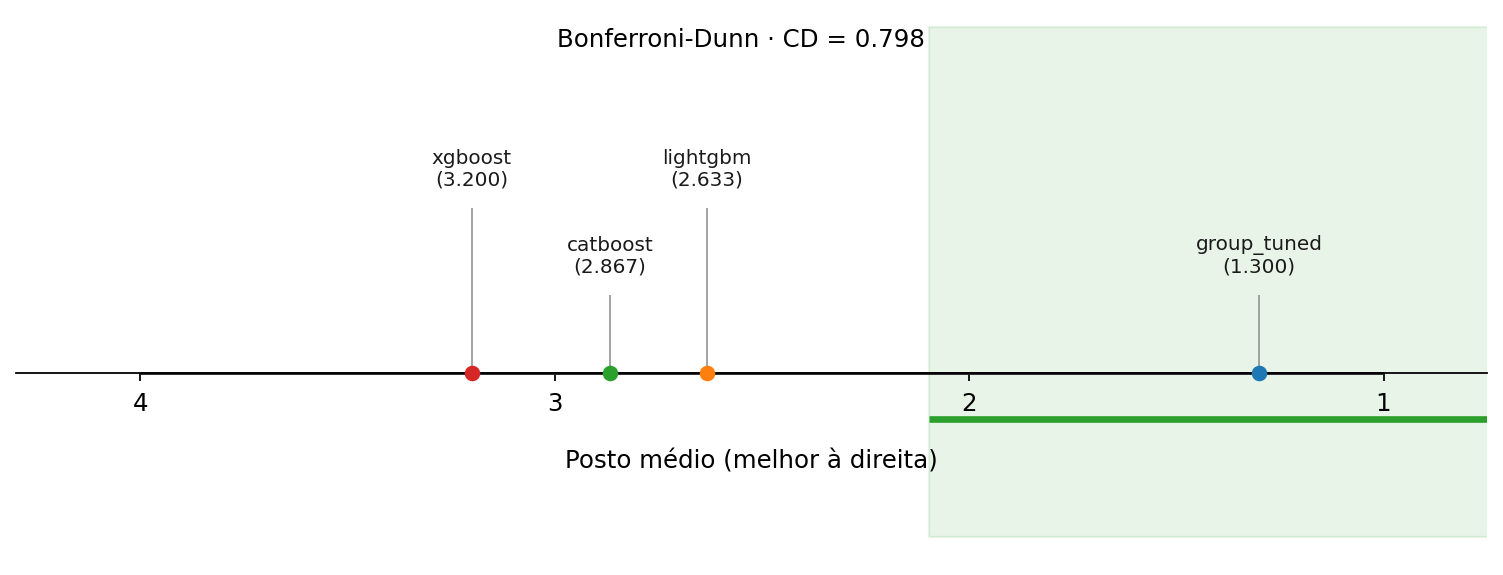
\includegraphics[width=\linewidth]{../figuras/cd_bonferroni_dunn_auc_ovo.png}
    \end{columns}
    \vspace{0.4em}
    \footnotesize \textbf{Conclusão:} o TabICL v2 supera \textbf{todos os 3 baselines} com significância estatística tanto por Holm ($p \le 6{,}33 \times 10^{-5}$) quanto por Bonferroni-Dunn em AUC OvO; na Entropia Cruzada, supera CatBoost e XGBoost por BD e todos os três por Holm ($p \le 0{,}0357$).
\end{frame}

% Slide 18: Nemenyi e diagrama CD
% Apresenta: integrante 4
\begin{frame}{Etapa 2: análise complementar (Nemenyi e diagrama CD)}
    \begin{columns}[T,onlytextwidth]
        \column{0.50\textwidth}
        \centering
        \textbf{\scriptsize Métrica primária: AUC OvO}\\[0.2em]
        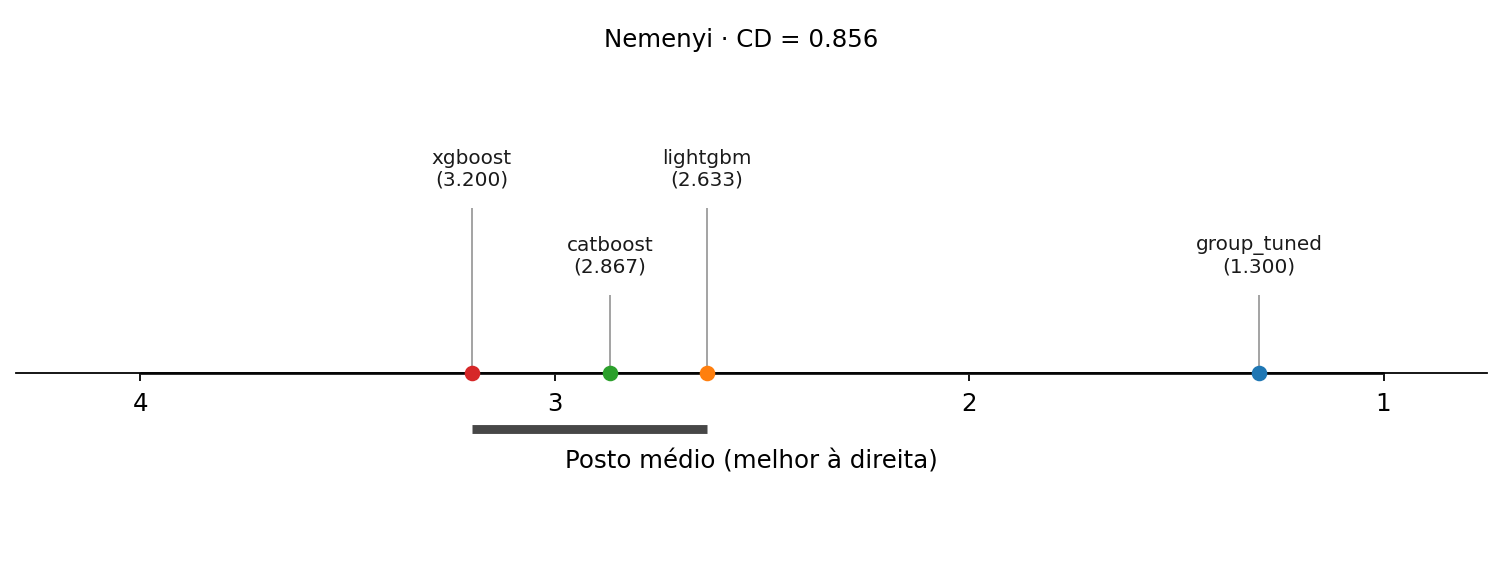
\includegraphics[width=\linewidth]{../figuras/cd_nemenyi_auc_ovo.png}
        \column{0.50\textwidth}
        \centering
        \textbf{\scriptsize Métrica secundária: Entropia Cruzada}\\[0.2em]
        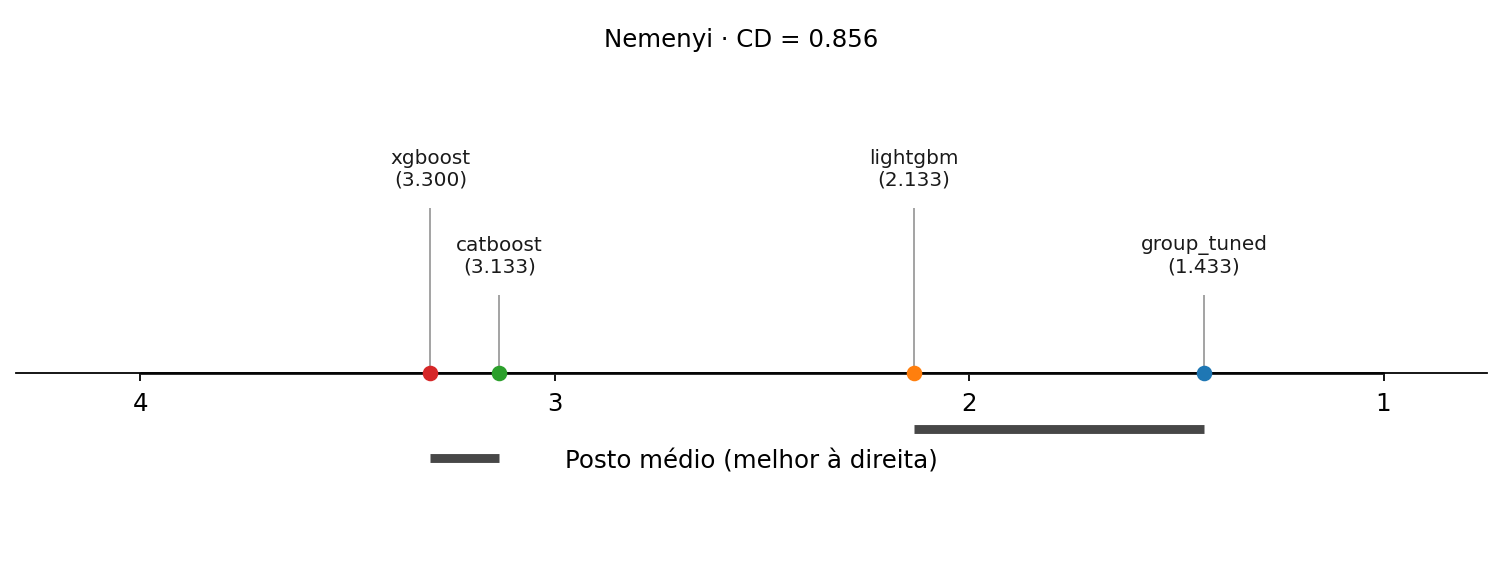
\includegraphics[width=\linewidth]{../figuras/cd_nemenyi_cross_entropy.png}
    \end{columns}
    \vspace{0.3em}
    \footnotesize \textbf{$\mathrm{CD}_{\mathrm{Nem}} = 0{,}856$} ($q_{0{,}05} = 2{,}569 \times 0{,}3333$, controlando $\binom{4}{2} = 6$ pares):
    \begin{itemize}
        \scriptsize
        \item \textbf{Em AUC OvO:} \texttt{group\_tuned} ($1{,}300$) fica \textbf{isolado em 1º lugar}; grupos sem diferença significativa (clique): \textbf{\{\texttt{lightgbm} ($2{,}633$), \texttt{catboost} ($2{,}867$), \texttt{xgboost} ($3{,}200$)\}} ($\Delta R_{\max} = 0{,}567 < 0{,}856$).
        \item \textbf{Em Entropia Cruzada:} grupos sem diferença significativa por Nemenyi: \textbf{\{\texttt{group\_tuned} ($1{,}433$), \texttt{lightgbm} ($2{,}133$)\}} e \textbf{\{\texttt{catboost} ($3{,}133$), \texttt{xgboost} ($3{,}300$)\}}, pois \texttt{lightgbm} passa a superar significativamente \texttt{catboost} ($\Delta R = 1{,}000 > 0{,}856$) e \texttt{xgboost} ($\Delta R = 1{,}167 > 0{,}856$).
    \end{itemize}
\end{frame}

% Slide 19: padrão vs. com busca
% Apresenta: integrante 3
\begin{frame}{Etapa 2: padrão vs.\ com busca (Wilcoxon)}
    \small
    \begin{itemize}
        \setlength{\itemsep}{2pt}
        \item \textbf{Diferenças usadas = 30 de $N = 30$:} em AUC OvO, $R^+ = 281{,}0$, $R^- = 184{,}0$, $T = 184{,}0$, $\mathbf{p = 0{,}3285}$ (não significativo); na Entropia Cruzada, $R^+ = 1{,}0$, $R^- = 464{,}0$, $T = 1{,}0$, $\mathbf{p = 3{,}725 \times 10^{-9}}$ a favor de \texttt{group\_default}.
        \item \textbf{Vitórias, empates e derrotas da variante com busca (\texttt{group\_tuned}):} $\mathbf{18 / 0 / 12}$ em AUC OvO ($0{,}8606$ vs.\ $0{,}8607$) e $\mathbf{1 / 0 / 29}$ em Entropia Cruzada (\texttt{group\_default} vence em 29/30 bases).
        \item \textbf{Custo da busca:} tempo mediano de $\mathbf{170{,}67\text{ s}}$ (média $196{,}49\text{ s}$, máx.\ $717{,}95\text{ s}$) por fold externo, multiplicando o tempo total por $\mathbf{9{,}84\times}$ ($218{,}78\text{ s}$ vs.\ $22{,}24\text{ s}$).
        \item \textbf{A busca compensa?} \textbf{Não.} O ganho em AUC é nulo ($p = 0{,}3285$), o tempo aumenta quase $10\times$ e a calibração/entropia cruzada piora significativamente em 29 dos 30 datasets.
        \item \textbf{Sensibilidade a 2 HPs e estudo específico (CV interna, notebook 03):} AUC OvO é quase plana em $\tau \in [0{,}5; 1{,}5]$ mas $\tau = 0{,}5$ infla a perda logarítmica ($0{,}5419 \to 0{,}6365$), explicando por que otimizar AUC prejudica CE; $\tau_{\mathrm{out}} \ge 4{,}0$, visões \texttt{["none","power"]} e $E=8$ confirmam o ótimo do padrão.
    \end{itemize}
\end{frame}

% Slide 20: análise por regime
% Apresenta: integrante 3
\begin{frame}{Etapa 2: análise por regime (descritiva)}
    \begin{columns}[T,onlytextwidth]
        \column{0.46\textwidth}
        \footnotesize
        \textbf{AUC OvO por regime de tamanho:}\\[0.3em]
        \resizebox{\linewidth}{!}{%
        \begin{tabular}{l c c c}
            \toprule
            \textbf{Sistema} & \textbf{Pequeno (10)} & \textbf{Médio (10)} & \textbf{Grande (10)} \\
            \midrule
            \textbf{TabICL v2 padrão}   & $\mathbf{0{,}8751}$ & $0{,}8615$ & $\mathbf{0{,}8455}$ \\
            \textbf{TabICL v2 c/ busca} & $\mathbf{0{,}8751}$ & $\mathbf{0{,}8618}$ & $0{,}8450$ \\
            LightGBM (TD)               & $0{,}8423$ & $0{,}8442$ & $0{,}8355$ \\
            CatBoost (TD)               & $0{,}8431$ & $0{,}8452$ & $0{,}8332$ \\
            XGBoost (TD)                & $0{,}8158$ & $0{,}8351$ & $0{,}8334$ \\
            \midrule
            \textbf{Vantagem TabICL}    & $\mathbf{+3{,}20\text{ p.p.}}$ & $\mathbf{+1{,}66\text{ p.p.}}$ & $\mathbf{+0{,}95\text{ p.p.}}$ \\
            \textbf{Posto médio TabICL} & $\mathbf{1{,}00}$ & $\mathbf{1{,}30}$ & $\mathbf{1{,}60}$ \\
            \bottomrule
        \end{tabular}%
        }
        \column{0.52\textwidth}
        \textbf{\footnotesize Síntese descritiva dos estratos:}\\[0.2em]
        \begin{itemize}
            \scriptsize
            \setlength{\itemsep}{2.5pt}
            \item \textbf{Regime de tamanho:} o TabICL v2 é invicto no regime pequeno ($10/10$ vitórias, posto $1{,}00$ e $+3{,}20\text{ p.p.}$); a vantagem decresce com $n$ ($+1{,}66$ no médio e $+0{,}95$ no grande), onde GBDTs ganham volume amostral.
            \item \textbf{Tipo de tarefa:} lidera tanto em binários ($0{,}8551$ vs.\ $0{,}8337$ do CatBoost, $N=24$) quanto em multiclasse ($0{,}8829$ vs.\ $0{,}8762$ do XGBoost, $N=6$).
            \item \textbf{Atributos categóricos:} mantém dianteira tanto com poucos categóricos ($<25\%$: $0{,}8759$ vs.\ $0{,}8524$, $N=15$) quanto com muitos ($\ge 25\%$: $0{,}8454$ vs.\ $0{,}8309$, $N=15$).
            \item \textbf{Dados ausentes:} maior robustez relativa com dados ausentes ($0{,}8837$ vs.\ $0{,}8614$ do LightGBM e $0{,}8117$ do XGBoost, $N=6$), graças à imputação no $\mathrm{TF}_{\mathrm{col}}$.
        \end{itemize}
    \end{columns}
    \vspace{0.3em}
    \footnotesize \textbf{Número de datasets por célula:} $N_{\text{cel}} \in \{6, 10, 15, 24\}$; \textbf{leitura apenas descritiva:} com amostras reduzidas ($N \le 10$), a diferença crítica de Nemenyi sobe para $\mathrm{CD}_{N=10} = 1{,}483$ e $\mathrm{CD}_{N=6} = 1{,}915$, impedindo testes formais por estrato sem inflar o erro Tipo I.
\end{frame}

% Slide 21: custo vs. desempenho
% Apresenta: integrante 2
\begin{frame}{Etapa 2: custo vs.\ desempenho}
    \centering
    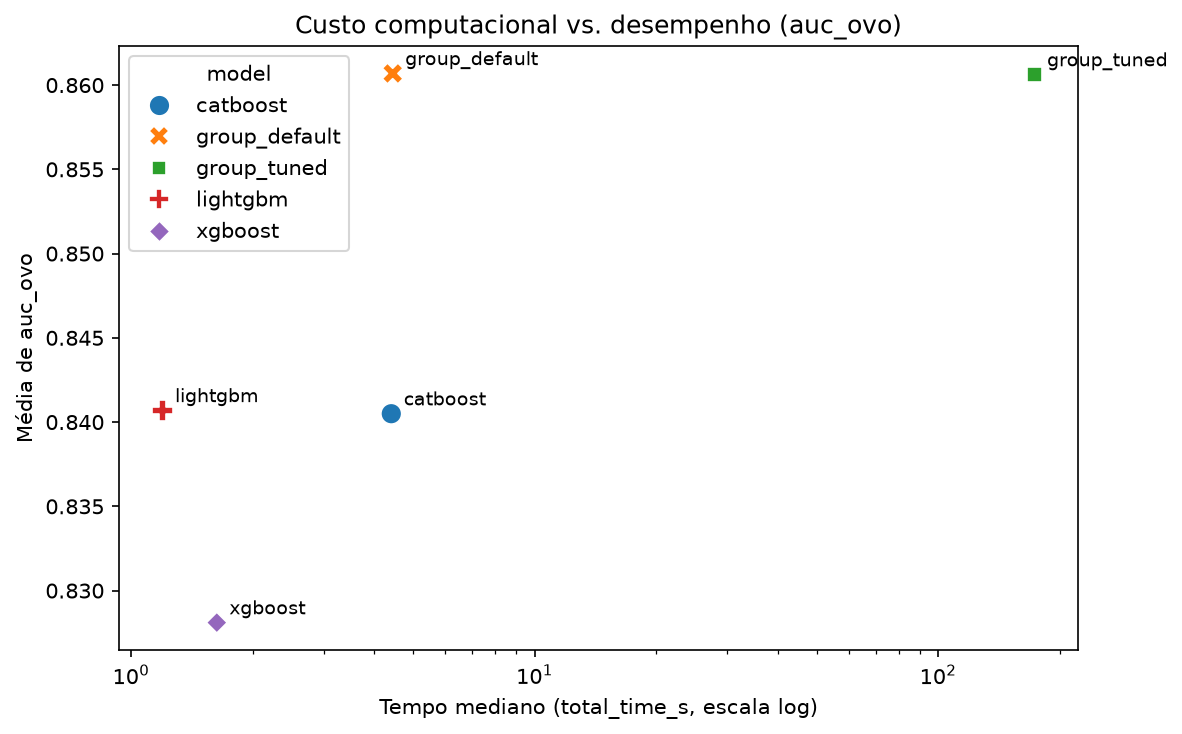
\includegraphics[height=4.4cm]{../../../results/figures/custo_vs_desempenho.png}
    \\[0.3em]
    \footnotesize \textbf{Posição do modelo do grupo na fronteira de Pareto:} \textbf{(1) Baixa latência em CPU ($3\text{--}5\text{ s}$):} \texttt{xgboost} ($2{,}96\text{ s}$, AUC $0{,}8281$) e \texttt{lightgbm} ($3{,}32\text{ s}$, AUC $0{,}8407$); \textbf{(2) Ótimo de Pareto em predição (\texttt{group\_default}, $22{,}24\text{ s}$ médios):} atinge a maior AUC ($0{,}8607$) e menor CE ($0{,}3005$) sem busca; e \textbf{(3) Dominado (\texttt{group\_tuned}, $218{,}78\text{ s}$):} custa $9{,}84\times$ mais sem ganho em AUC ($0{,}8606$).
\end{frame}

% Slide 22: pontos fortes, pontos fracos e ameaças à validade
% Apresenta: integrante 1
\begin{frame}{Etapa 2: pontos fortes, pontos fracos e ameaças à validade}
    \begin{itemize}
        \footnotesize
        \item \textbf{Melhor desempenho em:} datasets pequenos e médios ou com desbalanceamento/ausentes (exemplos: \texttt{Marketing\_Campaign} com $\mathbf{+0{,}0320}$ sobre LightGBM e $+0{,}3084$ sobre XGBoost; \texttt{Is-this-a-good-customer} com $\mathbf{+0{,}0610}$ sobre CatBoost; \texttt{maternal\_health\_risk} com $\mathbf{+0{,}0262}$ sobre XGBoost; e \texttt{polish\_companies\_bankruptcy} com $\mathbf{+0{,}0337}$ sobre CatBoost).
        \item \textbf{Pior desempenho em:} altíssima dimensionalidade esparsa com desbalanceamento extremo ou grandes tabelas com fronteiras simples (únicas 3 derrotas de \texttt{group\_tuned}: \texttt{hiva\_agnostic} com $\mathbf{-0{,}0226}$ vs.\ XGBoost, $0{,}4759$ vs.\ $0{,}4985$; \texttt{bank-marketing} com $\mathbf{-0{,}0069}$ vs.\ CatBoost; e \texttt{E-CommereShippingData} com $\mathbf{-0{,}0015}$ vs.\ LightGBM).
        \item \textbf{Causa provável:} o prior causal suave (SCMs/Sobolev) regulariza fortemente amostras pequenas sem sobreajustar, mas em \texttt{hiva\_agnostic} ($p=1.617$ colunas binárias esparsas, razão de desbalanceamento $88{,}33$) o agrupamento de atributos e a atenção densa diluem sinais raros que divisões de árvores isolam.
        \item \textbf{Ameaças à validade:} \textbf{(i) Assimetria de busca:} baselines usaram \textit{Tuned Defaults} fixos ($\texttt{tune\_time\_s}=0$), mas o sucesso de \texttt{group\_default} ($\texttt{tune\_time\_s}=0$, AUC $0{,}8607$) confirma que o ganho vem da arquitetura; \textbf{(ii) Imputação:} \texttt{ImputedClassifier} (ordinal + mediana com indicador binário de ausência) nos baselines vs.\ imputação nativa pela média sem indicador e visões normalizadas no TabICL; \textbf{(iii) Subamostragem:} teto $\texttt{MAX\_SAMPLES}=10.000$ limita GBDTs no regime grande; \textbf{(iv) Falhas/retomadas:} 4 retomadas (\texttt{--resume}, 2 folds finais de \texttt{363628} no Kaggle) afetam apenas tempos de parede; \textbf{(v) $N$ por regime ($6\text{--}15$)} e \textbf{estudos em um único fold externo (fold 0)}; e \textbf{(vi) Origem das faixas:} declarada a priori da literatura, mas otimizar AUC causou desalinhamento com a entropia cruzada.
    \end{itemize}
\end{frame}

% Slide 23: conclusões
% Apresenta: todos
\begin{frame}{Conclusões}
    \small
    \begin{itemize}
        \setlength{\itemsep}{3pt}
        \item \textbf{Posição do modelo:} o \textbf{TabICL v2} superou de forma estatisticamente significativa LightGBM, CatBoost e XGBoost nos $N=30$ datasets em \textbf{AUC OvO} ($F_F = 20{,}695, p = 3{,}28 \times 10^{-10}$, posto médio $\mathbf{1{,}300}, p_{\mathrm{Holm}} \le 6{,}33 \times 10^{-5}$) e em \textbf{Entropia Cruzada} ($F_F = 24{,}970, p_{\mathrm{Holm}} \le 0{,}0357$).
        \item \textbf{Pontos fortes:} desempenho \textit{zero-shot} --- \textbf{\texttt{group\_default} empatou em AUC com \texttt{group\_tuned}} ($0{,}8607$ vs.\ $0{,}8606$, $p=0{,}3285$), venceu em 29/30 datasets em Entropia Cruzada ($0{,}3005$ vs.\ $0{,}3150$), liderou em G-Mean ($0{,}6548$) e teve menor incerteza de bootstrap, sendo invicto nos pequenos (posto $1{,}00$).
        \item \textbf{Limites:} custo $\mathcal{O}(n p^2 + n^2)$ exige GPU de 16 GB e offload para $p > 500$ (latência média de $22{,}24\text{ s}$ vs.\ $3{,}32\text{ s}$ do LightGBM em CPU); perde em alta dimensão esparsa desbalanceada (\texttt{hiva\_agnostic}); pesos abertos (BSD-3-Clause).
        \item \textbf{Próximos passos:} adotar \texttt{group\_default} (ou $E=4$ via 1 EP) em produção; orientar buscas futuras por log-loss/Brier score; avaliar calibração formal (ECE/Platt) e testes bayesianos (Benavoli et al., 2017).
    \end{itemize}
\end{frame}

% Slide 24: encerramento
% Apresenta: todos
\begin{frame}{Obrigado}
    \centering
    \textbf{\Large Perguntas?}
    \\[0.8em]
    \footnotesize
    \textbf{Repositório:} \texttt{https://github.com/leticialevleitao/projetoAM20262Q2}\\
    {\scriptsize (criado a partir do template \texttt{projeto-final-IN1102-2026.2})}\\[0.5em]
    \textbf{Contato:} Douglas Araújo Silva (das7@cin.ufpe.br), Felipe Araújo de Lima (fal6@cin.ufpe.br), Letícia De Albuquerque S.\ Leitão (lasl@cin.ufpe.br)\\[0.6em]
    \textbf{Referências principais:}
    \begin{itemize}
        \scriptsize
        \item Qu, J., Holzmüller, D., Varoquaux, G., Le Morvan, M. (2025, 2026). \textit{TabICL (ICML 2025)} \& \textit{TabICLv2 (\texttt{arXiv:2602.11139v2})}.
        \item Erickson, N.\ et al. (2025). \textit{TabArena: A Living Benchmark for Machine Learning on Tabular Data (\texttt{arXiv:2506.16791})}.
        \item Holzmüller, D., Grinsztajn, L., Steinwart, I. (2024). \textit{Better by Default: Strong Pre-Tuned MLPs and Boosted Trees (\texttt{pytabkit}, NeurIPS)}.
        \item Dem\v{s}ar, J. (2006). \textit{Statistical Comparisons of Classifiers over Multiple Data Sets}. JMLR, 7, 1--30.
        \item Hastie, T., Tibshirani, R., Friedman, J. (2009). \textit{The Elements of Statistical Learning}, 2nd ed., Springer.
    \end{itemize}
\end{frame}

\end{document}
